\documentclass[tikz,border=12pt]{standalone}
\usepackage{fontspec}
\setmainfont{Segoe UI}
\usepackage{amsmath,amssymb}
\usepackage{tikz}

\usetikzlibrary{calc,arrows.meta}

\begin{document}
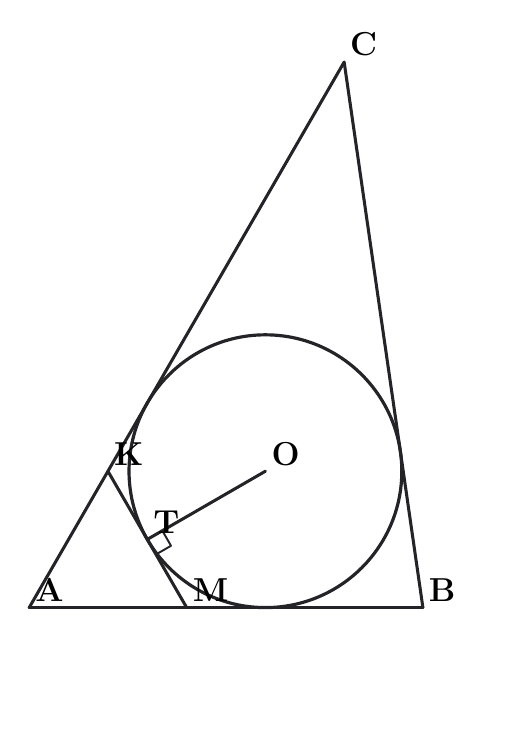
\begin{tikzpicture}[x=1.0000cm,y=1cm,line cap=round,line join=round]
\definecolor{linec0}{RGB}{35,35,40}
\definecolor{linec1}{RGB}{35,35,40}
\definecolor{linec2}{RGB}{35,35,40}
\definecolor{linec3}{RGB}{35,35,40}
\definecolor{linec4}{RGB}{35,35,40}
\definecolor{linec5}{RGB}{35,35,40}
\definecolor{edgecol}{RGB}{35,35,40}
\definecolor{hicol}{RGB}{35,35,40}
\definecolor{angcol}{RGB}{35,35,40}
\coordinate (A) at (0.0000,0.0000);
\coordinate (B) at (5.0000,0.0000);
\coordinate (C) at (4.0000,6.9282);
\coordinate (O) at (3.0000,1.7321);
\coordinate (M) at (2.0000,0.0000);
\coordinate (K) at (1.0000,1.7321);
\coordinate (T) at (1.5000,0.8660);
\draw[edgecol,line width=1.1pt] (A) -- (B);
\draw[edgecol,line width=1.1pt] (B) -- (C);
\draw[edgecol,line width=1.1pt] (C) -- (A);
\draw[edgecol,line width=1.1pt] (M) -- (K);
\draw[edgecol,line width=1.1pt] (O) -- (T);
\draw[edgecol,line width=1.15pt] (O) circle [x radius=1.7321, y radius=1.7321];
\path (0.068,-1.200) rectangle (5.932,4.664);
\draw[edgecol,line width=0.7pt] (1.691,0.976) -- (1.801,0.785) -- (1.610,0.675);
\node[font=\bfseries\large,inner sep=2pt,anchor=south west] at (0.000,0.000) {A};
\node[font=\bfseries\large,inner sep=2pt,anchor=south west] at (5.000,0.000) {B};
\node[font=\bfseries\large,inner sep=2pt,anchor=south west] at (4.000,6.928) {C};
\node[font=\bfseries\large,inner sep=2pt,anchor=south west] at (2.000,0.000) {M};
\node[font=\bfseries\large,inner sep=2pt,anchor=south west] at (1.000,1.732) {K};
\node[font=\bfseries\large,inner sep=2pt,anchor=south west] at (3.000,1.732) {O};
\node[font=\bfseries\large,inner sep=2pt,anchor=south west] at (1.500,0.866) {T};
\end{tikzpicture}
\end{document}
